\documentclass[a4paper,12pt]{article}
\usepackage[utf8x]{inputenc}
\usepackage{amssymb}
\usepackage{amsfonts}
\usepackage{mathrsfs}
\usepackage{amsmath}
\usepackage{amsthm}
\usepackage[margin=1.3cm]{geometry}
\usepackage{times}
\usepackage{graphicx}
\usepackage{enumitem}
\usepackage{fancyhdr}
\usepackage{hyperref}
\usepackage{setspace}
\usepackage{subcaption}
\usepackage{mathtools}
\usepackage[square,sort,comma,numbers]{natbib}
\setlength{\bibsep}{0.0pt}

%\pagestyle{fancy}
%\fancyhf{}
%\lhead{Thomas Delaney}
%\rhead{COSYNE 2018 Abstract}
%\cfoot{\thepage}

\newtheorem{theorem}{Theorem}
\newtheorem{proposition}{Proposition}[section]
\newtheorem{lemma}{Lemma}[section]
\newtheorem{corollary}{Corollary}[section]
\theoremstyle{definition}
\newtheorem{definition}{Definition}[section]

\newcommand{\boldnabla}{\mbox{\boldmath$\nabla$}} % to be used in mathmode
\newcommand{\cbar}{\overline{\mathbb{C}}}% to be used in mathmode
\newcommand{\diff}[2]{\frac{d #1}{d #2}}% to be used in mathmode
\newcommand{\difff}[2]{\frac{d^2 #1}{d #2^2}}% to be used in mathmode
\newcommand{\pdiff}[2]{\frac{\partial #1}{\partial #2}} % to be used in mathmode
\newcommand{\pdifff}[2]{\frac{\partial^2 #1}{\partial #2^2}}% to be used in mathmode
\newcommand{\upperth}{$^{\mbox{\footnotesize{th}}}$}%to be used in text mode
\newcommand{\vect}[1]{\mathbf{#1}}% to be used in mathmode
\newcommand{\curl}[1]{\boldnabla \times \vect{#1}} % to be used in mathmode
\newcommand{\divr}[1]{\boldnabla \cdot \vect{#1}} %to be used in mathmode
\newcommand{\modu}[1]{\left| #1 \right|} %to be used in mathmode
\newcommand{\brak}[1]{\left( #1 \right)} % to be used in mathmode
\newcommand{\comm}[2]{\left[ #1 , #2 \right]} %to be used in mathmode
\newcommand{\dop}{\vect{d}} %to be used in mathmode
\newcommand{\cov}{\text{cov}} %to be used in mathmode
\newcommand{\var}{\text{var}} %to be used in mathmode
\newcommand{\mb}{\mathbf} %to be used in mathmode
\newcommand{\bs}{\boldsymbol} %to be used in mathmode
% Title Page
\title{How informative are retinal ganglion cells?}
\author{Thomas Delaney 1330432}

\begin{document}

\noindent
\textbf{Title:} Does structure in neural correlations during spontaneous behaviour match anatomical structure?
\subsubsection*{300-word Summary}
Information in the brain is carried in correlated network activity. Decades of research has established that these correlations play a crucial role in representing sensory information\cite{cohen1}. Recent findings show that spontaneous behaviours can explain correlations in parts of the brain not usually related to motor control\cite{stringer}. In order to understand the brain, we must understand networks of correlated neurons. The question arises, are correlated networks restricted to anatomical brain regions?

Because of limitations in recording technology almost all research has explored correlations between neurons within a given brain region. Relatively little is known about correlations between neurons in different brain regions. However, the recent development of `Neuropixels' probes\cite{jun} has allowed extracellular voltage measurements to be collected from multiple brain regions simultaneously routinely, and in much larger numbers than traditional methods. In this project we used a publicly available Neuropixels dataset to analyse correlations between different brain regions.

Using eight probes each in three mice, readings from 2296, 2668, and 1462 cells respectively in nine different brain regions were extracted during approximately 1 hour of continuous activity. Each mouse was behaving spontaneously and could use their front paws to turn a wheel\cite{stringer}. Using these data, we examined pairwise spike count correlations between neurons within the same region, and between neurons in different regions. We found that cells from the same region tend to be more strongly correlated than cells from different regions. We also found that this difference in strength reduces when a longer time bin is used to bin spike counts.

We used a cutting-edge community detection method\cite{humphries} to detect communities in the network induced by pairwise correlations. We found that these communities generally exist across multiple brain regions. However, at shorter time-scales we found that communities dominated by cells from a single region were more prevelant. 

\subsubsection*{Additional Detail}
The three mice from which the data were collected had some key differences. The first mouse was a female wild type, P73. The second mouse was a male mutant (TetO-GCaMP6s, Camk2a-tTa), P113. The third mouse was a male mutant (Ai32, Pvalb-Cre), P99.

Prior to measuring spike count correlations, we chose suitable time bin widths for binning the spike counts by taking a similar approach to \cite{cohen2}. We evaluated the average correlations from many cell pairs using different values for the time bin width. We found that correlations increased logarithmically with the size of the bin width consistently across mice. We used a bin width of $2$s in order to capture the magnitude of the correlations, without completely averaging out short-term dynamics. However, we still performed our analyses at time bin widths ranging from $50$ms to $3$s in order to assess the effect of the bin width. The same dataset was used in \cite{stringer}, they used $1.2$s time bins for their analyses.

% revisit
To assess the correlation significance, we measured the shuffled correlation between each pair. We found that the mean correlation was usually an order of magnitude greater than the mean shuffled correlation. 

% disposable
% Due to the large number of cells, and the even larger number of cell pairs, in order to make these measurements in a reasonable amount of time, a local supercomputer was used to perform the calculations using parallelisation to speed up the process.

To compare \textit{within-region} mean correlations to \textit{between-region} mean correlations, we created correlation matrices with within-region correlations on the main diagonal and between-region correlations elsewhere. There appeared to be no consistency in correlation patterns across mice. % (see figure \ref{fig:regional_correlation_matrices}).

%\begin{figure}[t!]
%    \centering
%    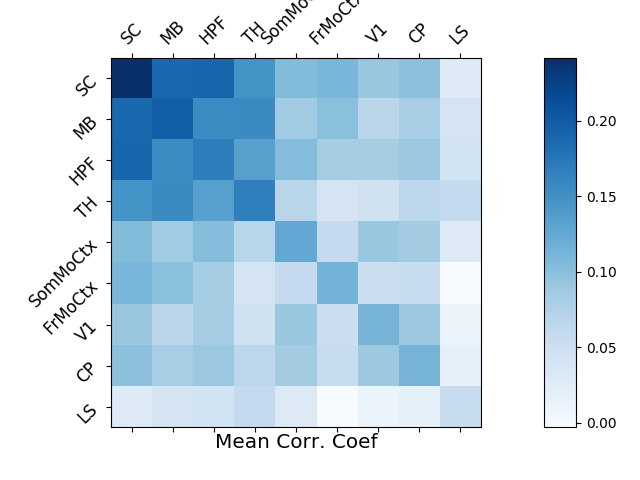
\includegraphics[width=0.32\columnwidth]{images/Krebs_2p0_corr.png}
%    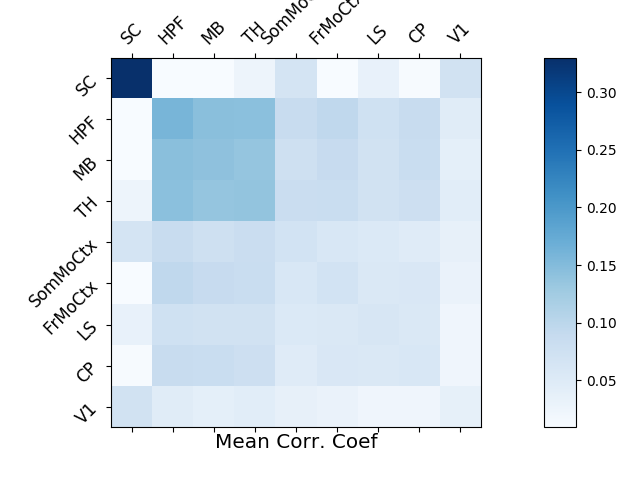
\includegraphics[width=0.32\columnwidth]{images/Robbins_2p0_corr.png}
%    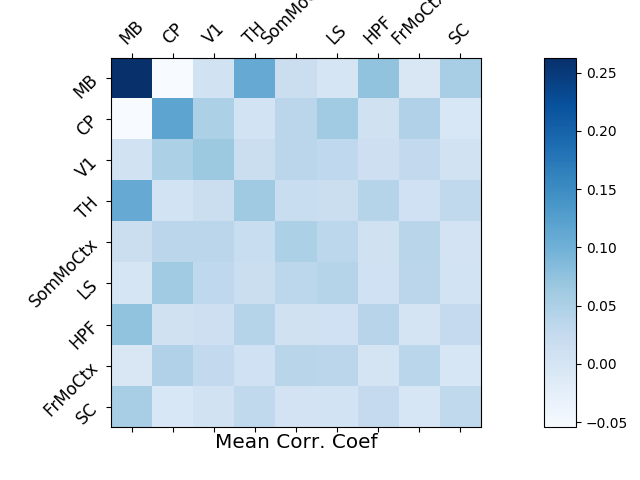
\includegraphics[width=0.32\columnwidth]{images/Waksman_2p0_corr.png}
%    \caption{Matrices showing the mean spike count correlation taken across pairs of neurons from various brain regions. One matrix for each mouse. Entries on the main diagonal correspond to pairs where each cell is from the same region. All other entries have pairs of cells from different regions.}
%    \label{fig:regional_correlation_matrices}
%\end{figure}

We compared within-region correlations to between-region correlations at different time-scales by using different values for the time bin width. For a given region, we found that within-region mean correlations tended to exceed most or all of the mean correlations for between-region correlations involving that region. We also found that this tendency was greatest for shorter time bins, and reduced for longer time bins (fig. \ref{fig:within_between}). This dynamic may reflect the dispersion of correlations throughout the brain over time.

\begin{figure}[t!]
    \centering
    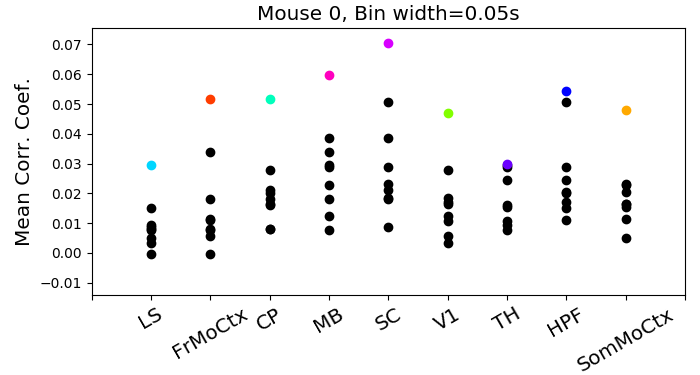
\includegraphics[width=0.45\columnwidth]{images/Krebs_0p05_corr_comp.png}
    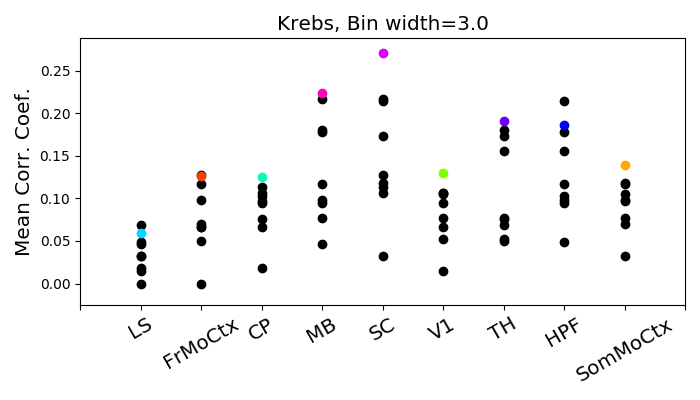
\includegraphics[width=0.45\columnwidth]{images/Krebs_3p0_corr_comp.png}
    \caption{Regional comparisons of within-region and between-region correlations for different time bin widths. The reduction in difference between within-region and between-region mean correlations was also observed at intermediate values for the time bin width.}
    \label{fig:within_between}
\end{figure}

The cutting-edge community detection method used involved choosing a null network distribution and testing if this model was valid for the data network. This hypothesis testing applied to network distributions allowed us to determine if the data network contained structure beyond that described by the null networks. It also allowed us to determine a subspace to the data network vector space where this structure exists, and which nodes contribute to this structure. Thus we could remove those nodes not contributing to the extra structure, and perform the community detection algorithm in the subspace. This process is referred to as \textit{Network Noise Rejection} \cite{humphries}. The community detection itself is analogous to ensemble methods for time-series analysis. It uses the output of many different modularity clustering attempts to find one final clustering through \textit{consensus-clustering}.

We performed the network noise rejection and community detection on weighted networks created by spike count correlation measurements. We did this using different values for the time bin width. We found that correlated communities generally included neurons from multiple brain regions. But, we found that communities dominated by neurons from a single region were more likely to be observed when using a smaller time bin width (fig. \ref{fig:regional_cluster_maps}). This result may also reflect dispersion of correlations throughout the brain over time.

\begin{figure}[t!]
    \centering
    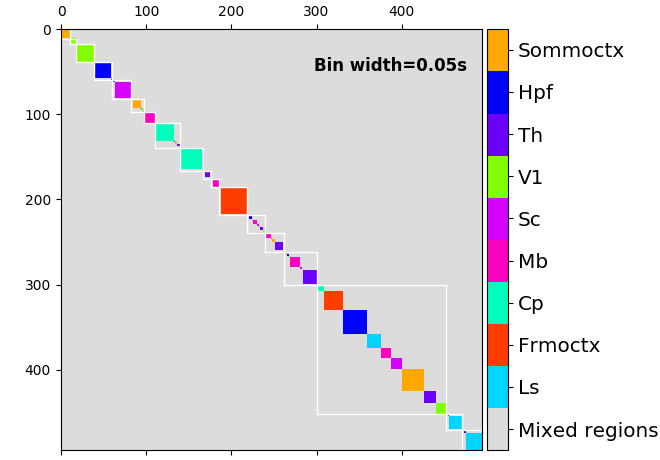
\includegraphics[width=0.45\columnwidth]{images/Krebs_0p05_regional_cluster_map.png}
    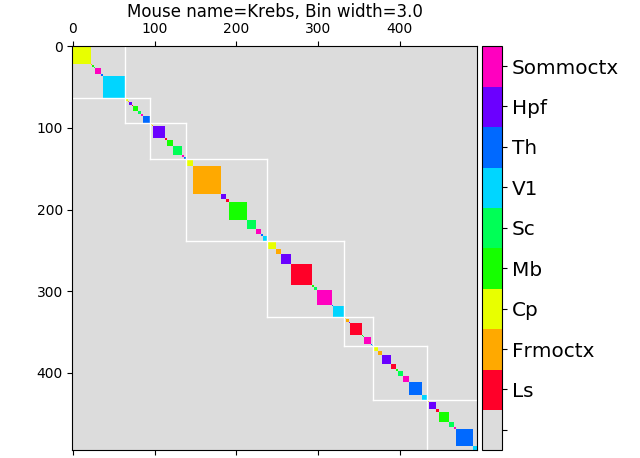
\includegraphics[width=0.45\columnwidth]{images/Krebs_3p0_regional_cluster_map.png}
    \caption{Matrices showing pairwise regional membership and correlation network community membership. Within-region pairs are coloured by their regional membership, between-region pairs are left grey. In general, communities include pairs from multiple regions. At shorter time-scales communities dominated by a single region are more prominent.}
    \label{fig:regional_cluster_maps}
\end{figure}



\bibliography{cosyne_2020_application.bbl}

%  \item correlation histogram results largely agree with previous findings, cite cohen and kohn.
\end{document}
